\documentclass[12pt, a4paper]{article}
\usepackage{float}
\usepackage[left=2cm, right=2cm, top=2cm, bottom=2cm]{geometry}
\usepackage{fancyvrb}
\usepackage{graphicx}
\usepackage{xeCJK}

\setCJKmainfont[AutoFakeBold=1.5]{新細明體}
\renewcommand{\arraystretch}{1.2}

\title{
  \vspace{-1cm}
  Network Administration/System Administration\\
  (NTU CSIE, Spring 2024)\\
  Lab 15 - Nmap \& Password Cracking
}
\author{\Large B12902110 呂承諺}

\setlength{\parindent}{0pt}

\begin{document}
  \maketitle

  \section{Nmap}
  \textbf{Steps}
  \begin{enumerate}
    \item SSH into the Kali VM from the Debian VM.
    \begin{Verbatim}[frame=single]
nasa2024@debian:~$ ssh -p 10022 localhost
    \end{Verbatim}
    \item Scan open ports on \verb|10.0.2.16| with Nmap.
    \begin{Verbatim}[frame=single]
nasa2024@kali-[~] $ nmap -v -sV -p1-65535 10.0.2.16
    \end{Verbatim}
  \end{enumerate}

  \textbf{Result}
  \begin{figure}[H]
    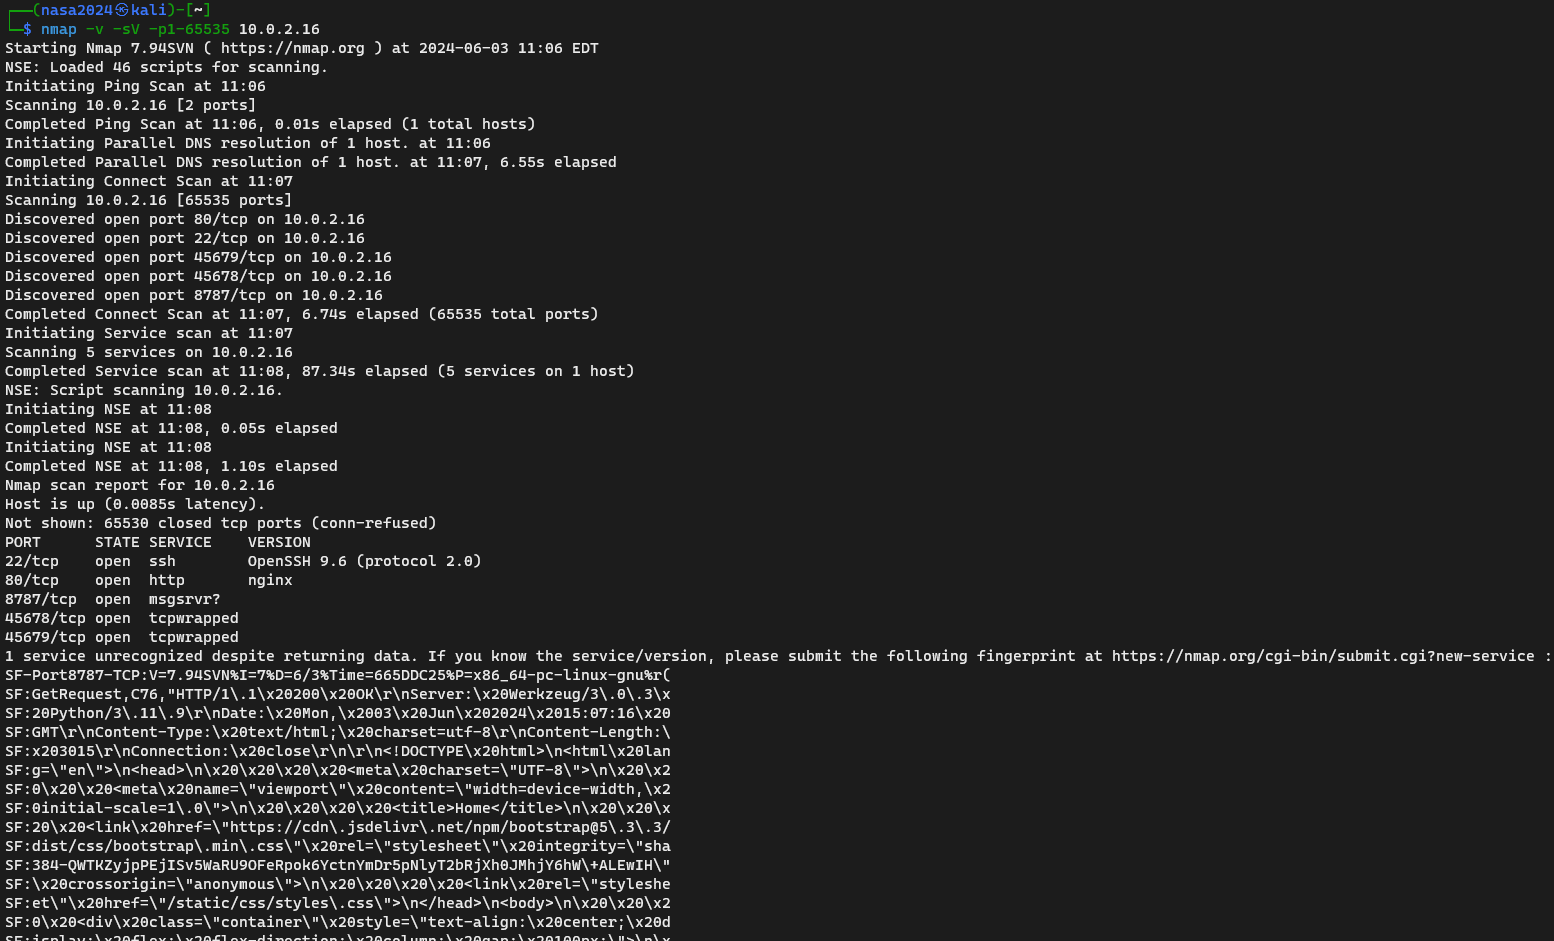
\includegraphics[width=\linewidth]{nmap.png}
  \end{figure}

  \section{Password Cracking}
  \textbf{Steps}
  \begin{enumerate}
    \item Access \verb|http://localhost:18787/| on the Debian VM. We
    see that user \verb|admin| has a hashed password of
    \verb|$2b$12$MUZRi07d.hFjdek1NPPbh.4G2SgpmpAnl6ZwhBNrtXqRK8hgJV8Da|.
    \item Save the password as a text file in the Kali VM.
    \begin{Verbatim}[frame=single]
nasa2024@kali-[~] $ echo \
  '$2b$12$MUZRi07d.hFjdek1NPPbh.4G2SgpmpAnl6ZwhBNrtXqRK8hgJV8Da' \
  > admin_password.txt
    \end{Verbatim}
    \item Unzip \verb|/usr/share/wordlists/rockyou.txt.gz|
    \begin{Verbatim}[frame=single]
nasa2024@kali-[/usr/share/wordlists] $ sudo gunzip rockyou.txt.gz
    \end{Verbatim}
    \item Use \verb|john| to crack the password.
    \begin{Verbatim}[frame=single]
nasa2024@kali-[~] $ john \
  --wordlist=/usr/share/wordlists/rockyou.txt \
  admin_password.txt
    \end{Verbatim}
    \item The cracked password is \verb|iloveyou4|. Use it to login to the website and
    obtain the flag.
  \end{enumerate}

  \textbf{Result}
  \begin{figure}[H]
    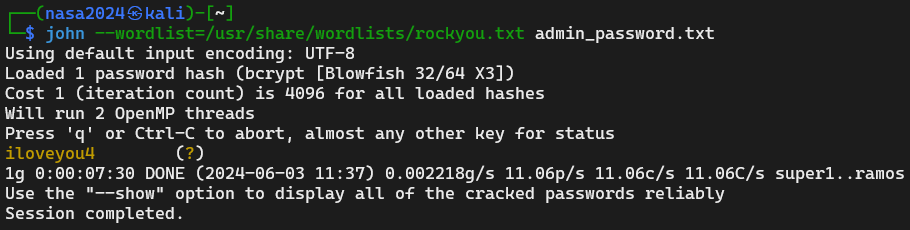
\includegraphics[width=\linewidth]{john.png}
  \end{figure}
  \begin{figure}[H]
    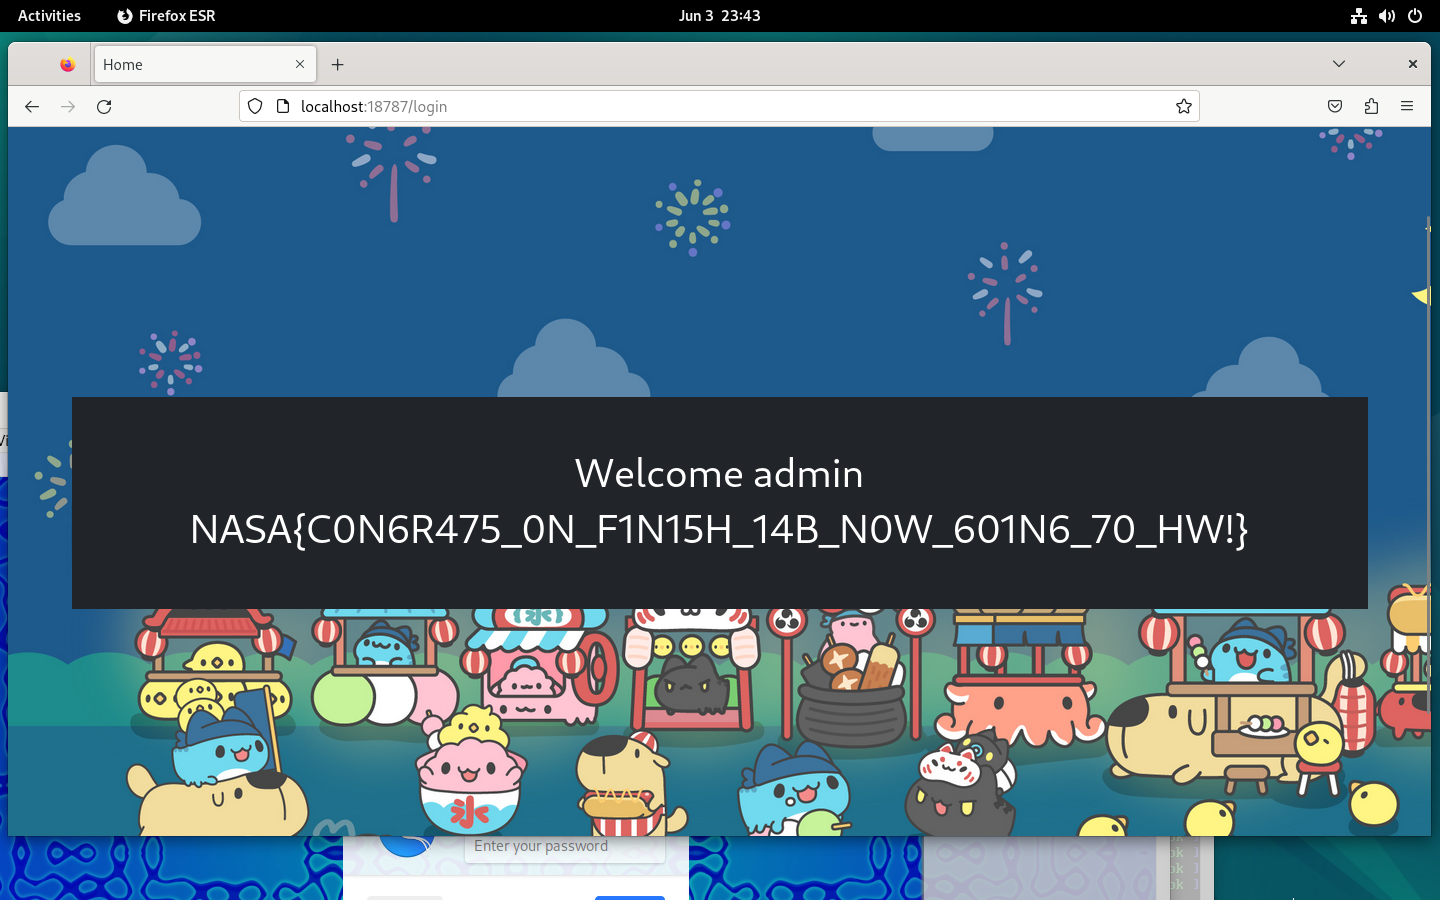
\includegraphics[width=\linewidth]{flag2.png}
  \end{figure}


\end{document}
